%% LyX 2.3.0 created this file.  For more info, see http://www.lyx.org/.
%% Do not edit unless you really know what you are doing.
\documentclass[english]{article}
\usepackage[T1]{fontenc}
\usepackage[latin9]{inputenc}
\usepackage{geometry}
\geometry{verbose,tmargin=2.5cm,bmargin=2.5cm,lmargin=2.5cm,rmargin=2.5cm}
\usepackage{graphicx}
\usepackage{babel}
\usepackage{listings}
\renewcommand{\lstlistingname}{Listing}

\begin{document}

\title{Favor Exchange}

\author{Chris A., ETH Zurich\\
Semion Rozov, ETH Zurich\\
KT Tan\\
Ivan Sergeev, ETH Zurich}
\maketitle

\section{Introduction}

The project we proposed for the open challenge of the BETH19 hackathon
revolves around social sustainability. We think that the way people
interact with each other online has been overly commercialized recently
(think about the thousand marketplaces, all the paid groups and paid
followers and bots on instagram and twitter) and would like to challenge
this common mindset.

This is why we wanted to create a platform where users could exchange
in a more sustainable and human way, primarily based on mutuality
and trust. Where people would come for help and to help out others.
People have many small tasks that need to be performed. For example,
helping out with groceries, delivering something, drilling a hole
in the wall or helping to assemble a piece of furniture. If they do
not have the time or the capacity to do this, they look for someone
to do it for them. We call these type of tasks favors. Asking for
a favor often comes with different issues. Often the payment is not
part of the process. This can make asking difficult or uncomfortable
if there is a refusal. Or, if one wants to pay for a small service
it can be difficult to estimate a fair price for it. For the other
party it might also feel awkward to accept cash for something he/she
would do for free. Secondly, these small tasks are supplied by people
in close nexus with the asker. It can happen that the Nexus of known
people is insufficiently large and so the number of people that can
be called on to do favours is limited.

Although there exist different similar projects which could tackle
the above problems, each of them has significant disadvantages in
comparison to our proposed solution: Craigslist, a classified advertisement
platform, is infamously known for scams, misleading advertisements
and generally raises safety concerns. A mobile app called Fiverr gives
users access to a freelance platform, which however operates in a
centralized manner and therefore can not convincingly guarantee user\textquoteright s
privacy or safety. Another centralized project called KISS tries to
solve the problem of elderly care in a sustainable way, but fails
to guarantee a reward to the current generation of caretakers due
to the large timescale of this project.

In contrast to the above, our vision is a DApp, which we called Favor,
that would allow users to exchange small favors for tokens and vice
versa. Instead of traditional currency, people would feel more comfortable
when returning or receiving something rather symbolic for the favor.
This symbolic value can be represented by a digital token living on
a blockchain. To keep it intuitively simple and away from the current
economic mindset, we fix a base rate of 1 real-world favor for 1 FVR
token. And because of this equivalence, favor incentivises its users
to help each other out as it guarantees them an equivalent \textquotedblleft good\textquotedblright{}
in return. We think that this can serve as a basis for other social
projects on the blockchain. However, in an ideal world, we would not
need the blockchain for that\dots{}

In this report, we will first go over the challenges and solutions
we faced during this project, explain the solution design in detail
and give an evaluation of the results. We finalize this report with
a brief conclusion and outlook.

\newpage{}

\section{Challenges and Solutions}

With Favor we try to solve the problems that most online exchange
platforms struggle with, which are Security and Fairness. Further
challenges we faced originate from the strict requirements that we
have set for this platform, all of which would make it scalable and
ready for immediate real world use. 

\subsection{Autonomy, security, and transparency}

We envision a decentralized and autonomous platform, which would have
the capability to record token transactions and contracts between
users in a secure way. All these requirements can be fulfilled with
a blockchain solution (in our case Ethereum), due to its immutable
and distributed nature: records of the transactions are kept in a
digital ledger, copies of which are maintained and validated by network
nodes. The validation of the transactions is designed to be inherently
difficult, so that it becomes computationally very difficult to introduce
falsifications. Thus, the functioning of such a network does not require
the supervision of a central authority, instead it requires agreement
and consistency between the network nodes. Further advantages of this
are that it is possible to ensure a fair token distribution and prevent
token inflation, which will be discussed shortly.

\subsection{Trust and cooperation}

Often, these are the main issues when users engage in online transactions.
How can one be sure that the other party will fulfill their task as
agreed and how can this be enforced? For this reason, our platform
features a commitment system that would disincentivize cheating and
unfair behavior and instead encourage users to cooperate. In order
to engage in a favor contract, users need to spend commitment tokens
which they get back after successful fulfillment of the contract.
This way, trust and cooperation can be established among users.

\subsection{Inflation and fair token distribution}

To prevent inflation effects, we decided to introduce new tokens into
the system as more users join. This keeps the token\textquoteright s
value inflation-proof.

However, the fair distribution has to be enforced additionally: It
is known, that many contemporary online platforms can be exploited
through botting or fake user accounts, especially if the platform
offers its users a signup bonus which may indirectly hold real monetary
value.

This is why we designed a special sign-up system: New users have to
earn their first FVR token by completing a task from a random list
(for stricter rules, a task that requires physical verification).
Their commitment token is granted by the smart contract, but only
released after a number of successful interactions.

It would be thus unreasonably difficult to sign up multiple accounts
with the goal of generating new tokens \textquotedblleft for free\textquotedblright .
Furthermore, a malicious user can not generate new tokens when completing
fictive favors with a network of bots, because the net balance in
the botnet would remain constant for the same number of bots (tokens
can not leave the botnet). The only way of introducing new tokens
would require signing up new bots, and thus more work, which would
be economically unreasonable.

\subsection{Symbolic value of tokens, free from commercial incentives}

We wanted to create a platform that would not involve any money at
any point. The exchange of tokens is completely untethered from any
currency, as the tokens value is strictly symbolic and essentially
represents a proof of physical human work. Furthermore, the limited
maximum wallet capacity makes over-the-counter selling (like in the
case of many ICOs) difficult and mostly useless. The only way to a
user can redeem a token is by requesting a favor from someone else.
This reassures the members that their helpfulness and good actions
will be returned to them in a similar way.

\subsection{User interaction design and the web application}

While the conceptual side of the project was quite challenging and
took many iterations to think through, we have also had to spend substantial
time on the UX design of the project. As none of us were skilled in
this are, we chose the most general HTML-CSS-JS approach and decided
to use a simple Web Application for the front-end instead of a dedicated
framework.

In summary, we can say that we have faced most of the above problems
for the first time, which allowed us to learn a lot about token economics
and sustainability and gain hands-on experience with the Ethereum
Blockchain as well as basic UX design.

\newpage{}

\section{Protocols}

\subsection{Exchange protocol}

The most basic exchange between a client and a provider entails the
provider completing a physical favor for the client and the client
transferring the agreed upon payment in tokens. However, this is only
possible in the ideal scenario when both parties act in good faith
and fulfill their part of the agreement. Indeed, a malicious client
might withhold payment for an already completed favor and a malicious
provider might ask for payment first and then refuse to perform the
favor. In both cases, the malicious party clearly gains a benefit,
either in the form of a physical favor or a token, at the expense
of the other party. To prevent such malicious behavior, the following
protocol is used for favor exchanges.
\begin{itemize}
\item Whenever a client creates a new favor request, the system deducts
two tokens from their account: one is the payment for the favor to
be completed and the other serves as a deposit.
\item When a provider agrees to complete the favor for the client, the system
also deducts one token from their account as a deposit.
\item Symmetrically, whenever a provider creates a new favor offer, they
automatically contribute one deposit token to the contract, and when
a client signs up to the agreement, their balance is reduced by two
tokens (again, payment plus deposit).
\item When both parties signal that the favor is complete, the system finalizes
the transaction by rewarding the provider with one token as payment
for the performed favor and returns the deposit tokens to both the
client and the provider. As a result, the net sum of the whole transaction
is a fair trade: one physical favor is performed by the provider for
the client and one token is transferred from the client to the provider.
\item Alternatively, if both parties agree to cancel the contract, all tokens
are refunded, so that both the client and the provider end up with
what they had initially. The option can be used, for example, if a
contract is created by mistake, if the favor cannot be completed by
the provider, or if the favor is no longer needed by the client.
\item Since some favors require more time and effort than others, the client
and provider can agree to exchange not one, but multiple tokens for
one physical favor. In this case, both parties are required to make
a deposit equal to the payment amount: if $x$ tokens are to be transferred
to the provider after the favor is performed, both the client and
the provider have to commit $x$ tokens as deposit to initiate the
contract (in addition to $x$ payment tokens contributed by the client
at contract initialization). To retain the symbolic value of tokens,
all payments are required to be integer.
\end{itemize}
Note that in this protocol the smart contract acts as an intermediary
between the client and the provider and its programming ensures that
the agreement is upheld by both parties. Since the transaction is
finalized only when consensus is reached (in the form of mutual consent
of the two parties), the cheating schemes described above are disincentivized.
If the client refuses to mark the contract as complete after the favor
is performed by the provider, they end up with a net loss of one token.
Similarly, if the provider refuses to complete the favor and does
not cancel the contract, they also lose one token as a result. To
sum up, the protocol facilitates fair exchanges of tokens for real-world
favors, allows cancellation of contracts by mutual agreement of both
parties, and prevents malicious behavior.

\subsection{Three-stage negotiation protocol}

In addition to ensuring fairness of favor exchanges, the system has
to manage information available to the users at each step of the exchange
process. On the one hand, revealing too much personal information
about the users or too many details about the favors might put the
privacy of the users at risk. On the other hand, insufficient or vague
information is an obstacle to developing trust and might cause disputes
between the parties. To combat these issues, we propose the following
three-stage negotiation protocol.
\begin{enumerate}
\item \textbf{Browsing stage.} Each user has access to the list of unmatched
favors, their basic descriptions and public information about other
users. However, for privacy protection, the information available
at this stage is limited, for example, only initials and generic locations
are accessible publicly, but not full names and precise locations.
Once a user finds a contract they are interested in, they can advance
to the next stage.
\item \textbf{Negotiation stage.} At this stage, the client and the provider
have the opportunity to stipulate the contract in more detail. Both
parties gain more access to each other's personal information and
can use an encrypted peer-to-peer channel for private communication.
Once the parties agree upon the terms of the contract, the exchange
protocol commences, the parties put their tokens into the smart contract,
and the process advances to the next stage. Otherwise, the contract
remains unmatched and the viewing user goes back to the browsing stage.
\item \textbf{Action stage.} Now that the exchange protocol commenced, it
is up to the provider to perform the favor for the client as agreed.
At this stage, the terms of the contract are transparent and trust
was developed between the client and the provider. As described above,
the exchange finishes when both parties agree that the favor is complete
or that the deal is called off.
\end{enumerate}
To conclude, this three-stage negotiation process strikes a perfect
balance between privacy at stage 1 and transparency at stage 3 while
giving both the client and the provider the ability to opt out at
stage 2.

\subsection{Initial token distribution}

Designing a token economy is a challenging task, even more so in our
case, since we set a number of additional requirements for our system.
First of all, the token economy should be decentralized, meaning that
there is no governing entity that distributes tokens and sets prices,
but instead, there is a free market economy influenced by the actions
of all the participants. Second, we would like to keep the token value
fixed and inflation-free: one should always be able to exchange 1
token for one real-world favor. Finally, the system should be able
to withstand botting attacks, when a single malicious party uses bots
to control multiple accounts, create dummy favors, and automatically
complete them, aiming to obtain an unlimited number of tokens for
free and then exchange them for real-world favors.

The additional requirements we set for the cryptoeconomic system significantly
limit the design space. For example, consider the strategy when new
tokens are minted and given to users after each successful favor exchange.
Even though this approach gives a decentralized dynamic-size economy,
it becomes practically infeasible under additional conditions. The
first issue is that inflation can only be prevented by carefully balancing
sources and sinks of cryptocurrency, which is a very delicate task.
Secondly, this this system is not bot-proof, because a botter can
earn an unlimited number of tokens for free by creating and completing
fake favors. The botting problem is especially severe, since tokens
obtained by bots can be used to request real-world favors basically
for free, effectively inflating the economy. Even though countermeasures
can be designed to combat these issues, the system remains fragile
and prone to abuse by malicious parties.

The cryptoeconomic system we propose is more robust, but less flexible
than the one described above. The total number of tokens in the economy
is strictly bound to the number of users, hence inflation is out of
the question. To seed the economy, a small number of users (e.g. the
first 100 to sign up on Favor Exchange) have their initial tokens
automatically unlocked and are able to use them freely from the start.
After the economy is seeded, every new user receives a small number
of tokens for free (say, 5), but they cannot exchange the initial
tokens for favors at first. Instead, the initial tokens are put into
an escrow, can only be utilized as deposit in exchange contracts (but
not as payment), and have to be ``unlocked'' by completing a certain
number of favors (for example, 5 for each token). This means that
the initial tokens represent a proof of work completed by the user,
and therefore token value does not decrease over time. Moreover, the
favors that the user has to complete to ``earn'' the initial tokens
are chosen from a small random list of (for instance, 10) unmatched
favors. This is done to prevent bot exploits, since the botter has
no control over the random favor requests they receive and thus cannot
reliably get the dummy favors in their selection. Note, however, that
this level of protection can be bypassed by creating a very large
number of duplicate accounts and/or complete favors. Since the botter
is likely to expend a large amount of resources on this brute force
method, we consider these countermeasures to be sufficient to disincentivize
malicious behavior.

\newpage{}

\section{Implementation}

\subsection{Overview}

The program consists of two parts: the back end --- a Solidity smart
contract --- and the front end --- a web client (HTML, CSS, JavaScript).
With the web client, users can create new favor requests and offers,
view available favors, sign up for the ones they are interested in,
and complete or cancel the contracts they participate in. Whenever
a favor is created, completed, or canceled by a user or personal information
is edited, the web client sends an appropriate query to the back end
via \lstinline!web3.js! functionality. Next, the smart contract processes
the query, applies changes to the data stored on the blockchain (if
necessary), and then sends the updated information back to the front
end. Finally, after receiving data from the back end, the web client
updates the contents of the webpage, and displays the updated information
to the user. Whenever any changes to the state of the blockchain are
made (e.g. a new favor is created), an event is emitted by the smart
contract and is processed by each web client, so all users always
stay up to date with the current state of affairs. The process is
summarized in the diagram shown on Figure 1.

\begin{figure}[h]
\begin{centering}
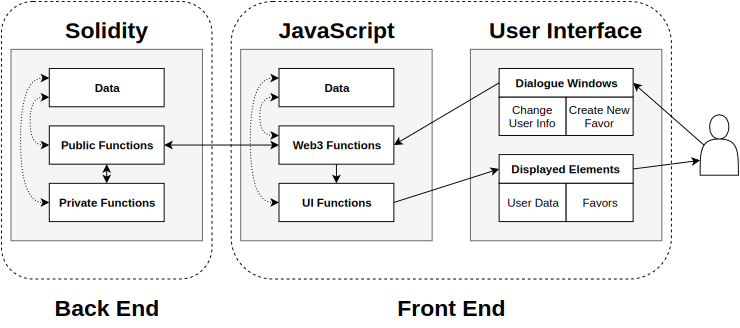
\includegraphics[width=1\textwidth]{architecture}
\par\end{centering}
\caption{Diagram of the architecture of the program. Dotted arrows represent
data transfers and solid arrows represent function calls and returns.}
\end{figure}


\subsection{Features}

The prototype we developed over the course of the hackathon is merely
a proof of concept rather than a finished product. Therefore, we aimed
to implement the following functionality, which lies at the core of
our solution:
\begin{itemize}
\item the information about the user and favors is stored and displayed;
\item the user is able to create, accept, cancel, and complete favors.
\end{itemize}
For the sake of simplicity and for testing purposes, purchase of favor
tokens via ether was implemented instead of the initial token distribution
protocol described above. Moreover, the second stage in the three-stage
negotiation process was omitted, reducing the scheme to its most primitive
form.

The version of the program submitted at the end of the hackathon (we
call it the Submitted Version from here on), the core functionality
was fully implemented at the back end level and partially at the front
end level with basic demonstration capabilities. A separate branch
of the GitHub repository contains an updated version (referred to
as the Updated Version), which features a finished front end that
fully demonstrates the intended core functionality of the solution.

\subsection{Known bugs}

In the Submitted Version, there is an issue with event handling: the
event handlers are called multiple times on a single event trigger,
even though the callback functions are bound via the \lstinline!event.watch()!
method as per Solidity documentation. In the Updated Version, this
issue is mitigated by using the \lstinline!allEvents()! method to
listen for events instead, but not resolved entirely: the latest event
trigger is processed again whenever the page is reloaded, even when
it is not required, which might sometimes lead to unexpected behavior.
Therefore, solving this problem requires more finesse in the setup
of event handling in a future version of the program.

\subsection{Future functionality}

The following important features are missing from the Submitted and
the Updated Versions of the program and are to be implemented in the
future.
\begin{itemize}
\item \textbf{Three-stage negotiation process.} This is one of the unique
aspects of our solution and should therefore be the top-priority feature
to be implemented in the future. It is not present in neither the
Submitted nor the Updated Version, since the concept was introduced
late into development and would require significant modifications
to the architecture of the program to be made. The negotiation stage
is especially tricky to add, since it relies on encrypted peer-to-peer
messaging, but the other two stages are straightforward to implement
within the existing framework.
\item \textbf{Initial token distribution.} This is also one of the key components
of our service and should be contained in the final product. The Submitted
and the Updated Versions allow purchase of tokens via ether, which
is suitable for testing purposes, but should be removed for the final
release.
\item \textbf{Improved UI.} Since the Submitted Version is the first prototype
of the program, the emphasis was put on implementing the core functionality.
In contrast, user experience should be the priority in the release
versions, and therefore improvements to the user interface of the
web client are required. Most importantly, the client-side functionality
should additionally include search and filter capabilities, which
are only present as a stub in the Submitted and the Updated Versions.
To augment user experience, new UI elements should be introduced,
such as a dashboard, tabs, and a user info viewer. Special attention
should be paid to styles and layout of the website to enhance visual
experience.
\item \textbf{Code improvements.} Should the project advance beyond the
prototype stage, more attention should be paid to code management.
To facilitate further development, the following practices (which
are industry standard) should be introduced: abiding by a strict code
style, writing detailed documentation, employing unit and integration
tests. In addition, the implementation of the favor token could be
changed to comply with an existing standard, such as ERC 20.
\item \textbf{Additional features. }The following features are not part
of the minimal viable product, but could potentially significantly
improve the system.
\begin{itemize}
\item \textbf{Reputation system.} To improve flexibility and increase social
interaction within the existing system, we should enable users to
provide feedback about the favor exchanges and other users. This could
be achieved by introducing a reputation score that represents dependability
of a user. Mechanically, reputation would be represented by a token
that is rewarded by other users after successful exchanges and that
could influence the order in which unmatched favors are listed for
other users, for example, as an additional sorting criterion.
\item \textbf{Less data on the blockchain.} In the Submitted and the Updated
Versions of the program, all the information about users and favors
is stored on the blockchain. Although this approach is acceptable
for the first prototype, it is infeasible in practice, since it is
associated with high costs. Thus information that is not essential
for secure storage and operation of agreements, such as users' personal
data and textual descriptions of completed favors, should be stored
in a database instead of on the blockchain.
\item \textbf{Distance calculation.} To improve user experience, the web
client should provide an estimate of the distance between the user
and the location where favor is requested or offered using an external
map service, since this information could be important at the negotiation
stage.
\item \textbf{User history.} Since the information about favor exchanges
is stored publicly on the blockchain, the users should have the ability
to access their and other users' full transaction history. This would
help make the system more transparent and trustworthy.
\end{itemize}
\end{itemize}
\newpage{}

\section{Conclusion and Outlook}

We believe this project serves as an example for the power of combinatorial
innovation, combining the advantages of existing services such as
Fiverr, Craigslist and social projects (KISS) and leveraging blockchain
technology to provide a decentralized service focused on fostering
sustainable behavior. We use short-term rewards to develop long-term
trust by incentivizing cooperation between users and disincentivizing
unfair usage.

The project was created with an emphasis on user security on one hand
and inhibiting automated gaming of the platform on the other hand.
In times of raised awareness for cyber crime, with enormous amounts
of time and money being -- rightfully -- spent on securing centralized
database systems, distributed ledger systems allow us to provide a
trustworthy and versatile platform to encourage sustainable behavior.
Through various precautionary measures, we believe we have made it
largely infeasible to use automated agents in order to gain an unfair
advantage on any larger scale. Furthermore, the personal security
of the users is enhanced through the reputation system and the fact
that we minimize the acute dependence of each user on any other specific
user, e.g. through providing choice to both providers and requesters.
This minimizes potential for coercion due to power imbalance.

From an implementation perspective, the project should be considered
as a successful proof of concept. More programming effort is needed
in order to make it a practical tool, however the prototype we\textquoteright ve
created was functional to a large extent and demonstrates the central
aspects of the application quite well.

The development tools employed in the prototype are mostly suited
to a development rather than a production setting. This is a limitation
that is not critical but would need to be taken into account for a
more serious implementation of the project. The technologies used
(i.e. ethereum blockchain, JavaScript, web app) seem to be the right
way to go. These are moderately to very well-established and provide
access to the application for a very wide audience. The only problematic
aspect from a user friendliness perspective would be the need to possess
an ethereum wallet and to acquire ether in order for any transaction
to be executed. We believe this issue will be mitigated as blockchain
technology becomes more and more widespread.

As explained under \emph{Initial Token Distribution}, the introduction
of liquidity into the ecosystem remains a challenge. This can be attributed
to some extent to the inherent problem of verification of physical
identity in the digital realm. We believe this is very much an unsolved
issue faced by many decentralized applications, as we have yet to
come across a reliable method for verifying statements about the physical
world in a decentralized way. Existing approaches tend to either provide
a quite unsatisfactory level of verification (e.g. community or sensor-based
verification), or leave the concrete mechanisms entirely unspecified
(using an oracle). We believe the approach we propose takes a reasonable
compromise between maximum security and user friendliness.

An important aspect of the proposed scheme is that the tokens are
strictly quantized, with a favor done being rewarded by an integer
number of FVR tokens. This leads to some desirable properties of the
currency: Firstly, it does not bear as much of a resemblance to money
(in fact it does not constitute money in the economic sense due to
this property), allowing for more moral freedom in its usage. Secondly
--- and supporting the first point --- it strengthens the decoupling
of the token currency from fiat currency. If the currency is quantized
in steps that are equal to the value of a typical transaction, it
becomes infeasible or at least unattractive to establish an exchange
rate of any sorts. Even though we have not had the chance to test
this on actual users, the idea has generally been well-received.

Our project suggests that a decentralized and community-driven ecosystem
focused on the exchange of minor favors purely for the sake of exchanging
favors (and being rewarded in favors) is feasible, from a technical
perspective as well as from an incentive-design perspective. As one
can easily verify through a quick survey of e.g. Craigslist ads, there
is also a market for such activities. One can imagine that the market
for favors that are not compensated in fiat currency would be larger
if anything, because of the multitude of use cases imaginable, some
of which may be far better suited to compensation via an abstract
reward system.
\end{document}
